%-*-coding:UTF-8-*-
%Fortran课作业
\documentclass[hyperref,UTF-8]{ctexart}
\hypersetup{colorlinks=false,pdfborder=000}
\usepackage{geometry}
\renewcommand{\rmdefault}{ptm}
\geometry{a4paper,centering,scale=0.88}
\title{\heiti 《FORTRAN语言》课作业及考试题目}
\author{\kaishu 王亮}
\date{\today}
\usepackage{multirow,makecell}
\usepackage{fancyvrb}
\usepackage{pifont}
\begin{document}
\zihao{4}
\maketitle
\tableofcontents
\begin{abstract}
这篇文档是《FORTRAN语言》课作业及考试题目,用\LaTeXe{}排版。建议使用高分辨屏幕阅读。
\end{abstract}
\section{数组、Fortran语言的格式输入和输出}
\subsection{题目1:计算差分表}
计算并在屏幕中输出下列差商表:其中x和f(x)为已知。
\begin{center}
\begin{tabular}{c|c|c|c|c|c|c}\hline
x&f(x)&&&&&\\\hline
0.40&0.41075&&&&&\\\hline
0.55&0.57815&1.11600&1.11600&&&\\\hline
0.65&0.69675&1.18600&0.28000&&&\\\hline
0.80&0.88811&1.27573&0.35893&0.19733&&\\\hline
0.90&1.02652&1.38410&0.43348&0.21300&0.3134& \\\hline
1.05&1.25382&1.51533&0.53493&0.22863&0.03126&0.00012 \\\hline
\end{tabular}
\end{center}

计算机源代码如下:

\begin{Verbatim}[numbers=left,commandchars=\\\{\},fontsize=\small]
!--THIS ARTICLE IS WRITTEN IN ANSI (GB18030)
!
!本程序读取数个二维坐标。这数个二维实数组是任意函数的部分点的横纵坐标,然后依据这些坐标,求其均差
!数据录入要求:数据应该放在一个程序能够有权限读取的顺序文件中。
!文件的每一行一个点的横纵坐标。第一个是横坐标,第二个是纵坐标
!本程序优秀之处:数据输出和输入全部使用文件;最大程度保护用户数据;录入数据可不按照大小顺序录入
!编写时间:2014年11月21日,作者:王亮
IMPLICIT NONE
!数据字典和变量申明
	INTEGER::i,j
	INTEGER::nvals=0
	INTEGER::status
	REAL::temp1,temp2
	LOGICAL::done
	CHARACTER(len=20)::filename
	REAL,ALLOCATABLE,DIMENSION(:,:)::a
!程序执行部分
!告知用户程序使用方法
WRITE(*,*)'==================================================================='
WRITE(*,*)'THIS PROGRAM IS SHOWN IN ANSI(GB18030)'
WRITE(*,*)'程序功能:本程序根据任意函数的部分点的横纵坐标,计算其均差。'
WRITE(*,*)'数据录入要求:数据应放在一个文件中。文件的每一行为一个点的横纵坐标。第一个是&
横坐标,第二个是纵坐标。'
WRITE(*,*)'编写时间:2014年11月21日,作者:王亮'
WRITE(*,*)'==================================================================='
!获取数据文件名称
WRITE(*,*)'现在,请键入输入文件名!文件名字符不得超过20个字符!'
READ(*,1000)filename
1000 FORMAT(A20)
!打开数据文件
OPEN(UNIT=1,FILE=filename,STATUS='OLD',ACTION='READ',IOSTAT=status)
!判断数据文件是否打开成功
IF(status==0) THEN !如果打开成功,数据录入给数组a
	!检索文件中数据,将文件中的实数个数赋值给nvals
	DO
		READ(1,*,IOSTAT=status) temp1,temp2
		IF(status/=0) EXIT
		nvals=nvals+1
	END DO
	!回到文件的开头
	REWIND(UNIT=1)
	!给可分配数组a确定其大小
	ALLOCATE(a(0:nvals-1,-1:nvals-1),STAT=status)
	IF(status/=0)THEN !如果出现数据过大等情况,告知用户内存不够而分配不成功,程序终止
		WRITE(*,*)'内存不足,程序终止'
		STOP
	END IF
	!如果文件能够成功打开且能将数据正常赋值给可分配数组,向用户回显原始数据
	WRITE(*,*)'文件打开成功,您输入的原始数据是'
	DO i=0,nvals-1
		READ(1,*) a(i,-1),a(i,0)
		WRITE(*,*)i,a(i,-1),a(i,0)
	END DO
ELSE!如果文件打开不成功,告知用户,并终止程序
	WRITE(*,*)'文件打开失败,程序终止!'
	STOP
END IF
WRITE(*,*)'您的原始数据共',nvals,'组','将计算到',nvals-1,'阶均差'
!用冒泡算法对数据按横坐标由小到大排序:在inner1循环中,检查i和i+1两个实数的大小,
!如果前者大就调换其顺序,
!循环i=1,navls-1对应第1个数据到倒数第二个(因为循环内命令出现i+1,所以最后一个
!数是参与比较了的,如果i=1,navls反而会造成越界错误)。
!outer1循环:不断执行inner1,以反复调换实数,当不存在需要调换情况时,done变量将保持真,
!被EXIT命令捕捉,退出循环。
!屏幕上输出结果
outer1: DO
	done=.TRUE.
	inner1:DO i=0,nvals-2
		IF(a(i,0)>a(i+1,0)) THEN
			temp1=a(i,-1)
			temp2=a(i,0)
			a(i,-1)=a(i+1,-1)
			a(i,0)=a(i+1,0)
			a(i+1,-1)=temp1
			a(i+1,0)=temp2
			done=.FALSE.
		END IF
	END DO inner1
	IF(done)EXIT
END DO outer1
WRITE(*,*)'调序完成:'
DO i=0,nvals-1		
	WRITE(*,*)i, a(i,-1),a(i,0)
END DO
WRITE(*,*)'==============================='
WRITE(*,*)'计算完成!'
WRITE(*,*)'==============================='
!下面的outer2循环是本程序的核心代码,核心代码仅5行
!outer2循环计算的是第j阶均差的结果。
!inner2循环计算的各阶均差的结果,依据就是均差的定义式
!注意:a循环存放输入数据和输出数据。行:0开始,列:-1开始。
!前两列放的是输入数据,之后的部分放入输出数据
!输出数据放入的元素是按照均差表排序的
!本算法的缺点是如果计算n个数据点的均差,会浪费1/2×(n×(n-1))各元素的内存,浪费率几乎为一半
outer2: DO j=1,nvals-1
	WRITE(filename,*)j
	WRITE(*,*)'#',TRIM(ADJUSTL(filename)),'阶差商结果开始'
	inner2: DO i=j,nvals-1
		a(i,j)=(a(i,j-1)-a(i-1,j-1))/(a(i,-1)-a(i-j,-1))
		WRITE(*,*)a(i,j)
	END DO inner2
	WRITE(*,*)'#',TRIM(ADJUSTL(filename)),'阶差商结果结束'
END DO outer2
!询问用户是否输出文件,最大程度保护计算结果,直到明确用户用途才关闭程序
DO
	WRITE(*,*)'是否需要将文件输出为文件?y/Y=是,n/N=否'
	READ(*,*)filename
	IF( (filename=='y').OR.(filename=='Y') )EXIT
	IF( (filename=='n').OR.(filename=='N') )THEN
		WRITE(*,*)'您输入的是',TRIM(ADJUSTL(filename)),'。程序结束,再见!'
		STOP
	ELSE 
		WRITE(*,*)'您输入的是',TRIM(ADJUSTL(filename))
		WRITE(*,*)'本程序只能接受y/Y或者n/N'
		WRITE(*,*)'为了保护数据,除非按规则输入,程序不会正常停止!'
	END IF
END DO
!询问用户输出文件的输出名,创建数据文件,并且最大程度保护计算结果和其他数据
DO
	WRITE(*,*)'请键入输出结果文件名。文件名不超过20个字符'
	READ(*,*)filename
	OPEN(UNIT=3,FILE=filename,STATUS='NEW',ACTION='READWRITE',IOSTAT=status)
	IF(status==0) THEN !如果打开成功,数据录入给数组a
		WRITE(*,*)'文件创建成功!'
		DO j=1,nvals-1
			WRITE(filename,*)j
			WRITE(3,*)'#',TRIM(ADJUSTL(filename)),'阶差商结果开始'
			DO i=j,nvals-1
				WRITE(3,*)a(i,j)
			END DO
			WRITE(3,*)'#',TRIM(ADJUSTL(filename)),'阶差商结果结束'
		END DO
		WRITE(*,*)'数据存储完成,程序结束,再见!'
	ELSE!如果文件打开不成功,告知用户重新输入文件名
		WRITE(*,*)'文件创建失败,可能是已经存在同名文件或文件夹'
		WRITE(*,*)'为保护数据,除非输入可以使用的文件,程序才正常结束'
	END IF
	IF(status==0) EXIT
END DO
END PROGRAM
\end{Verbatim}

本程序有以下亮点:
\begin{dinglist}{47}
\item 数据输出和输入全部使用文件。
\item 最大程度确保数据录入的正确和保护用户已有的文件。
\item 录入数据可不按照大小顺序录入,程序自动排序。
\end{dinglist}

计算机终端中使用gfortran编译,并运行:

\begin{Verbatim}[numbers=left,fontsize=\small]
C:\Users\wangliang\Documents\Fortran\王亮作业\第一次课>gfortran -o jieshang jies
hang.f95

C:\Users\wangliang\Documents\Fortran\王亮作业\第一次课>jieshang
 ===================================================================
 THIS PROGRAM IS SHOWN IN ANSI(GB18030)
 程序功能:本程序根据任意函数的部分点的横纵坐标,计算其均差。
 数据录入要求:数据应放在一个文件中。文件的每一行为一个点的横纵坐标。第一个是横
坐标,第二个是纵坐标。
 编写时间:2014年11月21日,作者:王亮
 ===================================================================
 现在,请键入输入文件名!文件名字符不得超过20个字符!
jieshang.txt
 文件打开成功,您输入的原始数据是
           0  0.400000006      0.410750002
           1  0.550000012      0.578149974
           2  0.649999976      0.696749985
           3  0.800000012      0.888109982
           4  0.899999976       1.02652001
           5   1.04999995       1.25381994
 您的原始数据共           6 组将计算到           5 阶均差
 调序完成:
           0  0.400000006      0.410750002
           1  0.550000012      0.578149974
           2  0.649999976      0.696749985
           3  0.800000012      0.888109982
           4  0.899999976       1.02652001
           5   1.04999995       1.25381994
 ===============================
 计算完成!
 ===============================
 #1阶差商结果开始
   1.11599982
   1.18600059
   1.27573299
   1.38410079
   1.51533306
 #1阶差商结果结束
 #2阶差商结果开始
  0.280003101
  0.358929634
  0.433471203
  0.524929166
 #2阶差商结果结束
 #3阶差商结果开始
  0.197316334
  0.212975934
  0.228644922
 #3阶差商结果结束
 #4阶差商结果开始
   3.13192047E-02
   3.13379802E-02
 #4阶差商结果结束
 #5阶差商结果开始
   2.88853298E-05
 #5阶差商结果结束
 是否需要将文件输出为文件?y/Y=是,n/N=否
y
 请键入输出结果文件名。文件名不超过20个字符
jieshangresult.txt
 文件创建成功!
 数据存储完成,程序结束,再见!
\end{Verbatim}
\subsection{题目2:数据排序}
用选择排序法5,3,6,4,8,7,1,9,2,10从小到大进行排序。

计算机源代码如下:

\begin{Verbatim}[numbers=left,commandchars=\\\{\},fontsize=\small]
PROGRAM sort
!--THIS ARTICLE IS WRITTEN IN ANSI(GB18030)
!
!本程序读取一个实数数据组,然后把这些数由小到大排列。
!数据录入要求:数据应该放在一个程序能够有权限读取的顺序文件中,其每一行应为一个实数。
!
!编写时间:2014年11月7日,作者:王亮
IMPLICIT NONE
!数据字典和变量申明
	INTEGER::i
	INTEGER::nvals=0
	INTEGER::status
	REAL::temp
	LOGICAL::done
	CHARACTER(len=20)::filename
	REAL,ALLOCATABLE,DIMENSION(:)::a
!程序执行部分
!告知用户程序使用方法
WRITE(*,*)'==================================================================='
WRITE(*,*)'程序功能:本程序读取一个实数数据组,然后把这些数由小到大排列。'
WRITE(*,*)'数据录入要求:数据应该放在一个程序有权限读取的文件名小于20个字符的顺序文件中,&
其每一行应为一个实数。'
WRITE(*,*)'编写时间:2014年11月7日,作者:王亮'
WRITE(*,*)'==================================================================='
!获取数据文件名称
WRITE(*,*)'现在,请输入文件名!'
READ(*,1000)filename
1000 FORMAT(A20)
!打开数据文件
OPEN(UNIT=1,FILE=filename,STATUS='OLD',ACTION='READ',IOSTAT=status)
!判断数据文件是否打开成功
IF(status==0) THEN !如果打开成功,数据录入给数组a
	!检索文件中数据,将文件中的实数个数赋值给nvals
	DO
		READ(1,*,IOSTAT=status) temp
		IF(status/=0) EXIT
		nvals=nvals+1
	END DO
	!回到文件的开头
	REWIND(UNIT=1)
	!给可分配数组a确定其大小
	ALLOCATE(a(1:nvals),STAT=status)
	IF(status/=0)THEN !如果出现数据过大等情况,告知用户内存不够而分配不成功,程序终止
		WRITE(*,*)'内存不足,程序终止'
		STOP
	END IF
	!如果文件能够成功打开且能将数据正常赋值给可分配数组,向用户回显原始数据
	WRITE(*,*)'文件打开成功,您输入的原始数据是'
	DO i=1,nvals
		READ(1,*) a(i)
		WRITE(*,*)i,a(i)
	END DO
ELSE!如果文件打开不成功,告知用户,并终止程序
	WRITE(*,*)'文件打开失败,程序终止!'
	STOP
END IF
!用冒泡算法计算结果:在inner循环中,检查i和i+1两个实数的大小,如果前者大就调换其顺序,
!循环i=1,navls-1对应第1个数据到倒数第二个(因为循环内命令出现i+1,所以最后一个
!实数是参与比较了的,如果i=1,navls反而会造成越界错误)。
!outer循环:不断执行inner,以反复调换实数,当不存在需要调换情况时,done变量将保持真,被EXIT命令捕捉,退出循环。
outer: DO
	done=.TRUE.
	inner:DO i=1,nvals-1
		IF(a(i)>a(i+1)) THEN
			temp=a(i)
			a(i)=a(i+1)
			a(i+1)=temp
			done=.FALSE.
		END IF
	END DO inner
	IF(done)EXIT
END DO outer
!屏幕上输出结果
WRITE(*,*)'计算完成,结果是'
DO i=1,nvals		
	WRITE(*,*)i, a(i)
END DO
END PROGRAM sort
\end{Verbatim}

本程序有以下亮点:
\begin{dinglist}{47}
\item 数据输入使用文件。
\item 不拘泥于题目要求的数据,体现数据与程序分离的编程思想。
\item 自动识别数据输入数目,不需用户告知。
\end{dinglist}

计算机终端中使用gfortran编译,并运行:

\begin{Verbatim}[numbers=left,fontsize=\small]
C:\Users\wangliang\Documents\Fortran\王亮作业\第一次课>gfortran -o sort sort_ans
i.f95

C:\Users\wangliang\Documents\Fortran\王亮作业\第一次课>sort
 ===================================================================
 程序功能:本程序读取一个实数数据组,然后把这些数由小到大排列。
 数据录入要求:数据应该放在一个程序有权限读取的文件名小于20个字符的顺序文件中,
其每一行应为一个实数。
 编写时间:2014年11月7日,作者:王亮
 ===================================================================
 现在,请输入文件名!
sort.txt
 文件打开成功,您输入的原始数据是
           1   10.0000000
           2   20.0000000
           3   30.0000000
           4   30.0000000
           5   0.00000000
           6   9.80000019
           7   1000.00000
           8  -9.00000000
           9  -500.000000
          10   26.7000008
          11   78.0000000
          12   95.0999985
 计算完成,结果是
           1  -500.000000
           2  -9.00000000
           3   0.00000000
           4   9.80000019
           5   10.0000000
           6   20.0000000
           7   26.7000008
           8   30.0000000
           9   30.0000000
          10   78.0000000
          11   95.0999985
          12   1000.00000
\end{Verbatim}
\section{分支结构和循环结构}
\subsection{题目1:学生成绩分类}
将学生成绩分为优、良、中、及格和不及格5个档次,从键盘中输入学生的成绩,程序输出对应的档次。

计算机源代码如下:

\begin{Verbatim}[numbers=left,commandchars=\\\{\},fontsize=\small]
IMPLICIT NONE
	REAL::i
	INTEGER::j
WRITE(*,*)'==================================================================='
WRITE(*,*)'THIS PROGRAM IS SHOWN IN ANSI(GB18030)'
WRITE(*,*)'程序功能:学生成绩分类程序'
WRITE(*,*)'成绩应在0到100之间。90-100为优,80-89为良,70-79为中,&
60-69为及格,低于60为不及格。'
WRITE(*,*)'编写时间:2014年11月27日,作者:王亮'
WRITE(*,*)'==================================================================='
WRITE(*,*)'请输入成绩'
READ(*,*,IOSTAT=j)i
IF(j==0)THEN
	IF((i>=90).AND.(i<=100))THEN
		WRITE(*,*)'成绩为优'
	ELSE IF((i>=80).AND.(i<90))THEN
		WRITE(*,*)'成绩为良'
	ELSE IF((i>=70).AND.(i<80))THEN
		WRITE(*,*)'成绩为中'
	ELSE IF((i>=60).AND.(i<70))THEN
		WRITE(*,*)'成绩为及格'
	ELSE IF((i>=0).AND.(i<60))THEN
		WRITE(*,*)'成绩为不及格'
	ELSE
		WRITE(*,*)'输入的数字不在0到100'
	END IF
ELSE
	WRITE(*,*)'输入的不是数字'
END IF
WRITE(*,*)'程序结束'
END PROGRAM
\end{Verbatim}

本程序有以下亮点:
\begin{dinglist}{47}
\item 如果用户输入非法(不是数字),程序可识别,告知用户,体现主动捕捉异常,防止程序不正常结束,即所谓的“茁壮代码”的编程思想。
\end{dinglist}

计算机终端中使用gfortran编译后运行:

\begin{Verbatim}[numbers=left,fontsize=\small]
C:\Users\wangliang\Documents\Fortran\王亮作业\第二次课>a
 ===================================================================
 THIS PROGRAM IS SHOWN IN ANSI(GB18030)
 程序功能:学生成绩分类程序
 成绩应在0到100之间。90-100为优,80-89为良,70-79为中,60-69为及格,低于60为不及
格。
 编写时间:2014年11月27日,作者:王亮
 ===================================================================
 请输入成绩
95
 成绩为优
 程序结束
\end{Verbatim}
\subsection{题目2:小球反弹}
已知某球从100m高度自由落下,落地后反复弹起。每次弹起的高度是上次高度的一半。求此球第10次落地后反弹起的高度和球所经过的路程。

计算机源代码如下:

\begin{Verbatim}[numbers=left,commandchars=\\\{\},fontsize=\small]
IMPLICIT NONE
	INTEGER::i,j,r!i是反弹次数,j是读取正确判断用变量,r是循环计数器
	REAL(KIND=4)::h,s,temp!h是一次的路程,s是总路程
WRITE(*,*)'==================================================================='
WRITE(*,*)'THIS PROGRAM IS SHOWN IN ANSI(GB18030)'
WRITE(*,*)'本程序是小球反弹作业'
WRITE(*,*)'编写时间:2014年11月27日,作者:王亮'
WRITE(*,*)'==================================================================='
WRITE(*,*)'请输入高度'
READ(*,*,IOSTAT=j)h
IF(.NOT.(j==0))THEN
	WRITE(*,*)'输入值非实数,程序结束。'
	STOP
END IF
IF(h<=0)THEN
	WRITE(*,*)'输入了非正数,程序结束。'
	STOP
END IF
WRITE(*,*)'请输入反弹次数'
READ(*,*,IOSTAT=j)i
IF(.NOT.(j==0))THEN
	WRITE(*,*)'输入值非整数,程序结束。'
	STOP
END IF
IF(i<=0)THEN
	WRITE(*,*)'输入值非正数,程序结束。'
	STOP
END IF
s=h
DO r=1,i
	h=h/2
	temp=(s+(2*h))
	IF(s==temp)THEN
		WRITE(*,*)'因为精度原因,计算提前结束'
		WRITE(*,*)'程序计算到了第',r-1,'次碰撞'
	END IF
	IF(s==temp)EXIT
	s=temp
	write(*,*)h,s
END DO
WRITE(*,*)'最后一次反弹高度是',h,'总的路程是',s-h
WRITE(*,*)'程序结束'
END PROGRAM
\end{Verbatim}

本程序有以下亮点:
\begin{dinglist}{47}
\item 不拘泥高度和反弹次数必须是100和10,用户可自由输入数据。
\item 如果用户输入非法(如不是数字或正数),程序可识别,告知用户,体现主动捕捉异常,防止程序不正常结束,即所谓的“茁壮代码”的编程思想。
\item 如果计算次数过高,超过计算机精度,程序采用不依赖于处理机的方式识别,并停止运算,告知用户计算情况。
\end{dinglist}

计算机终端中使用gfortran编译后运行:

\begin{Verbatim}[numbers=left,fontsize=\small]
C:\Users\wangliang\Documents\Fortran\王亮作业\第二次课>gfortran -o b 2.f95

C:\Users\wangliang\Documents\Fortran\王亮作业\第二次课>b
 ===================================================================
 THIS PROGRAM IS SHOWN IN ANSI(GB18030)
 本程序是小球反弹作业
 编写时间:2014年11月27日,作者:王亮
 ===================================================================
 请输入高度
100
 请输入反弹次数
10
 最后一次反弹高度是   9.76562500E-02 总的路程是   299.707031
 程序结束
\end{Verbatim}
\section{子程序和子函数编写}
\subsection{题目1:计算自然对数底数e的近似值}
设计一个计算n!的子程序,并调用该程序计算数e的近似值。计算公式为:
$$e=1+\frac{1}{1!}+\frac{1}{2!}+\dots +\frac{1}{n!}+\dots $$
当$n!>10^8$时停止计算(第一组用函数子程序编,第三组用子例行程序编,第四组用内部子程序编,第五组用递归调用编)。

计算机源代码存于数个文件中。

主程序存于1.f95文件中:

\begin{Verbatim}[numbers=left,commandchars=\\\{\},fontsize=\small]
!--THIS ARTICLE IS WRITTEN IN ANSI(GB18030)--
!
!本程序计算数e的近似值。计算公式为:
!e=1+1/1!+1/2!+……+1/n!+……
!
!本程序使用了函数子程序、子例行程序、内部子程序和递归方法分别计算。当n!>1E8时停止计算。
!
!本程序编译时应包含1.f95(本文件)、digui.f95、sub.f95和fun.f95,若用gfortran编译,命令为:
!gfortran 1.f95 digui.f95 sub.f95 fun.f95
!
!编写时间:2014年12月4日,作者:王亮
IMPLICIT NONE
INTEGER(KIND=8)::n,result
INTEGER::fun
REAL(KIND=8)::e
WRITE(*,*)'==================================================================='
WRITE(*,*)'THIS PROGRAM IS SHOWN IN ANSI(GB18030)'
WRITE(*,*)'程序功能:计算e的近似值。计算公式为:e=1+1/1!+1/2!+……+1/n!+……'
WRITE(*,*)'编写时间:2014年12月4日,作者:王亮'
WRITE(*,*)'==================================================================='
!====函数子程序方法======
e=0.
n=0
result=0
DO
	result=fun(n)
	e=e+(1/REAL(result))!包括其他三种计算方法:为避免整型变量和&
	实型变量的除法混合计算,用REAL转换函数处理
	IF(result>1e8)EXIT
	n=n+1
END DO
WRITE(*,*)'函数子程序方法'
WRITE(*,*)'e='
WRITE(*,*)e
!====函数子程序方法======
!====子例行程序方法======
e=0.
n=0
result=0
DO
	CALL sub(n,result)
	e=e+(1/REAL(result))
	IF(result>1e8)EXIT
	n=n+1
END DO
WRITE(*,*)'子例行程序方法'
WRITE(*,*)'e='
WRITE(*,*)e
!====子例行程序方法======
!====内部子程序方法======
e=0.
n=0
result=0
DO
	result=jiechen(n)
	e=e+(1/REAL(result))
	IF(result>1e8)EXIT
	n=n+1
END DO
WRITE(*,*)'内部子程序方法'
WRITE(*,*)'e='
WRITE(*,*)e
!====内部子程序方法======
!====递归方法======
e=0.
n=0
result=0
DO
	CALL factorial(n,result)
	e=e+(1/REAL(result))
	IF(result>1e8)EXIT
	n=n+1
END DO
WRITE(*,*)'递归方法'
WRITE(*,*)'e='
WRITE(*,*)e
!====递归方法======
CONTAINS
	INTEGER FUNCTION jiechen(n)
	INTEGER(KIND=8)::i,j,n
	j=1
	DO i=1,n
		j=j*i
	END DO
	jiechen=j
	END
END
\end{Verbatim}

函数子程序代码存于fun.f95中:

\begin{Verbatim}[numbers=left,commandchars=\\\{\},fontsize=\small]
!--THIS ARTICLE IS WRITTEN IN ANSI(GB18030)--
INTEGER FUNCTION fun(n)
IMPLICIT NONE
	INTEGER(KIND=8)::i,j,n
j=1
DO i=1,n
	j=j*i
END DO
fun=j
END
\end{Verbatim}


子例行程序代码存于sub.f95中:

\begin{Verbatim}[numbers=left,commandchars=\\\{\},fontsize=\small]
!--THIS ARTICLE IS WRITTEN IN ANSI(GB18030)--
SUBROUTINE sub(n,result)
IMPLICIT NONE
INTEGER(KIND=8)::i
INTEGER(KIND=8),INTENT(IN)::n
INTEGER(KIND=8),INTENT(OUT)::result
result=1
DO i=1,n
	result=result*i
END DO
END SUBROUTINE
\end{Verbatim}

递归子程序的代码存于digui.f95中:

\begin{Verbatim}[numbers=left,commandchars=\\\{\},fontsize=\small]
!--THIS ARTICLE IS WRITTEN IN ANSI(GB18030)--
RECURSIVE SUBROUTINE factorial(n,result)
IMPLICIT NONE
INTEGER(KIND=8),INTENT(IN)::n
INTEGER(KIND=8),INTENT(OUT)::result
INTEGER(KIND=8)::temp
IF(n>=1)THEN
	CALL factorial(n-1,temp)
	result=n*temp
ELSE
	result=1
END IF
END SUBROUTINE factorial
\end{Verbatim}

代码经编译运行结果如下:

\begin{Verbatim}[numbers=left,fontsize=\small]
C:\Users\wangliang\Documents\Fortran\王亮作业\第三次课>gfortran 1.f95 digui.f95
sub.f95 fun.f95

C:\Users\wangliang\Documents\Fortran\王亮作业\第三次课>a
 ===================================================================
 THIS PROGRAM IS SHOWN IN ANSI(GB18030)
 程序功能:计算e的近似值。计算公式为:e=1+1/1!+1/2!+……+1/n!+……
 编写时间:2014年12月4日,作者:王亮
 ===================================================================
 函数子程序方法
 e=
   2.7182818282861687
 子例行程序方法
 e=
   2.7182818282861687
 内部子程序方法
 e=
   2.7182818282861687
 递归方法
 e=
   2.7182818282861687

\end{Verbatim}

本程序有以下亮点:
\begin{dinglist}{47}
\item 使用了四种方法进行计算,超额完成任务
\end{dinglist}
\subsection{题目2:调用子程序和子函数进行计算}
分别调用子程序和子函数程序计算:
$$sum=\sqrt{x^3+y^4} +tan(x^2+y^2)$$

主程序源代码存放于2.f95文件中:
\begin{Verbatim}[numbers=left,commandchars=\\\{\},fontsize=\small]
!--THIS ARTICLE IS WRITTEN IN ANSI(GB18030)--
!
!本程序计算计算sum=sqrt(x^3+y^4)+tan(x^2+y^2)
!
!本程序编译时应包含2.f95(本文件)、tan.f95和sqrt.f95,若用gfortran编译,命令为:
!gfortran 2.f95 sqrt.f95 tan.f95
!
!编写时间:2014年12月4日,作者:王亮
IMPLICIT NONE
	REAL::a,b,x,y,mytan
	INTEGER::j
WRITE(*,*)'==================================================================='
WRITE(*,*)'THIS PROGRAM IS SHOWN IN ANSI(GB18030)'
WRITE(*,*)'程序功能:计算sum=sqrt(x^3+y^4)+tan(x^2+y^2)'
WRITE(*,*)'编写时间:2014年12月4日,作者:王亮'
WRITE(*,*)'==================================================================='
WRITE(*,*)'请输入x'
READ(*,*,IOSTAT=j)x
IF(.NOT.(j==0))THEN
	WRITE(*,*)'输入的不是数字'
	WRITE(*,*)'程序结束'
	STOP
END IF
WRITE(*,*)'请输y'
READ(*,*,IOSTAT=j)y
IF(.NOT.(j==0))THEN
	WRITE(*,*)'输入的不是数字'
	WRITE(*,*)'程序结束'
	STOP
END IF
IF((x**3+y**4)<0)THEN
	WRITE(*,*)'负数不能开方'
	WRITE(*,*)'程序结束'
	STOP
END IF
IF(ABS((x**2+y**2)-3.14159)<0.0001)THEN
	WRITE(*,*)'k*pi+pi/2无正切值'
	WRITE(*,*)'程序结束'
	STOP
END IF
		CALL mysqrt(a,x,y)
b=mytan
WRITE(*,*)a+b
END PROGRAM
\end{Verbatim}

子程序的源代码存放于sqrt.f95中:

\begin{Verbatim}[numbers=left,commandchars=\\\{\},fontsize=\small]
SUBROUTINE mysqrt(a,x,y)
IMPLICIT NONE
REAL,INTENT(IN)::x,y
REAL,INTENT(OUT)::a
a=sqrt(x**3+y**4)
END
\end{Verbatim}

子函数的源代码存放于tan.f95中:
\begin{Verbatim}[numbers=left,commandchars=\\\{\},fontsize=\small]
REAL FUNCTION mytan(x,y)
IMPLICIT NONE
REAL,INTENT(IN)::x,y
mytan=TAN(x**2+y**2)
END FUNCTION
\end{Verbatim}

编译运行结果:

\begin{Verbatim}[numbers=left,fontsize=\small]
C:\Users\wangliang\Documents\Fortran\王亮作业\第三次课>gfortran -o b 2.f95 sqrt
f95 tan.f95

C:\Users\wangliang\Documents\Fortran\王亮作业\第三次课>b
 ===================================================================
 THIS PROGRAM IS SHOWN IN ANSI(GB18030)
 程序功能:计算sum=sqrt(x^3+y^4)+tan(x^2+y^2)
 编写时间:2014年12月4日,作者:王亮
 ===================================================================
 请输入x
10
 请输y
9
   86.9540100
\end{Verbatim}
本程序有以下亮点:
\begin{dinglist}{47}
\item 如果用户输入非法(如不是数字),程序可识别,告知用户,体现主动捕捉异常,防止程序不正常结束,即所谓的“茁壮代码”的编程思想。
\item 充分考虑了用户输入值可能造成无法开方和无正切值的情况。
\end{dinglist}
\section{文件操作}
\subsection{题目1:向文件写入字符串}
把字符串“Hello Fortran”按照顺序存取和直接存取的方式分别存入3种文件结构中,并比较三种文件结构的区别。

计算机源代码如下:
\begin{Verbatim}[numbers=left,commandchars=\\\{\},fontsize=\small]
!--THIS ARTICLE IS WRITTEN IN ANSI(GB18030)--
!
!本程序向三种文件,两种方式输出Hello FORTRAN。
!
!编写时间:2014年12月16日,作者:王亮
OPEN (10,FILE='FS.txt' ,FORM='FORMATTED',ACCESS='SEQUENTIAL') 
WRITE(10,*)'Hello FORTRAN'
OPEN (11,FILE='FD.txt' ,FORM='FORMATTED',ACCESS='DIRECT',RECL=50) 
WRITE(11,'(A)',rec=1)'Hello FORTRAN'
OPEN(12,FILE='US.txt',FORM='UNFORMATTED',ACCESS='SEQUENTIAL')
WRITE(12)'Hello FORTRAN'
OPEN (13,FILE='UD.txt' ,FORM='UNFORMATTED',ACCESS='DIRECT',RECL=50) 
WRITE(13,REC=1)'Hello FORTRAN'
OPEN (14,FILE='C.txt' ,FORM='BINARY',ACCESS='SEQUENTIAL') 
WRITE(14)'Hello FORTRAN'
OPEN (14,FILE='D.txt' ,FORM='BINARY',ACCESS='DIRECT',RECL=50) 
WRITE(14,REC=1)'Hello FORTRAN'
END
\end{Verbatim}

程序编译运行后,即会产生对应的文件。

\noindent
对它们进行对比,有如下几点结论:
\begin{enumerate}
\item FS.txt即是平时用的普通的所谓的文本文件,用文本编辑器如Windows记事本等打开可以看到程序输入的字符串“Hello Fortran”。
\item FD.txt是有格式的直接存取的文件,用文本编辑器如Windows记事本等打开可以看到程序输入的字符串“Hello Fortran”。
\begin{itemize}
\item 如果改变“REC=”子句的参数,可以看到记录的位置随之改变。
\end{itemize}
\item  US.txt是FORTRAN语言中所谓的无格式文件,但若用文本编辑器如Windows记事本等打开,依然可以看到程序输入的字符串“Hello Fortran”。这是因为即使是所谓的无格式,要存储一个字符串依然需要一定的编码格式,所以依然可以打开。
\item  UD.txt是FORTRAN语言中所谓的无格式文件,并且使用直接存取的方式,若用文本编辑器如Windows记事本等打开,可以看到程序输入的字符串“Hello Fortran”。和US.txt相同,这是因为即使是所谓的无格式,要存储一个字符串依然需要一定的编码格式,所以依然可以打开。
\begin{itemize}
\item 如果向直接存取文件输出数字,用文本编辑器打开则不会正确显示。注意:不一定是“乱码”,只是不正确显示,因为可能是刚好某个可识别的字符,比如在我的机器上实验如果输出数字100,则刚好显示字符“d”。
\end{itemize}
\item  D.txt和 D.txt是BINARY文件,并且使用直接存取的方式,若用文本编辑器如Windows记事本等打开,可以看到程序输入的字符串“Hello Fortran”。
\end{enumerate}
\subsection{题目2:删除文件程序}
编写一个程序,要求输入一个文件名称,判断这个文件是否存在,如果存在就把它删除,不存在就显示错误信息。

源代码如下:

\begin{Verbatim}[numbers=left,commandchars=\\\{\},fontsize=\small]
!--THIS ARTICLE IS WRITTEN IN ANSI(GB18030)--
!
!本程序要求输入一个文件名称,判断这个文件是否存在,如果存在就把它删除,不存在就显示错误信息。
!
!编写时间:2014年12月16日,作者:王亮
IMPLICIT NONE
	CHARACTER(len=20)::filename,err_str
	INTEGER::i
WRITE(*,*)'请输入文件名,此文件将被删除!'
READ(*,*)filename
OPEN(UNIT=1,FILE=filename,STATUS='OLD',IOSTAT=i)
IF (i==0)THEN
	CLOSE(UNIT=1,STATUS='DELETE',IOSTAT=i)
ELSE
WRITE(*,*)'错误,没有这个文件'
END IF
END
\end{Verbatim}

编译运行:

\begin{Verbatim}[numbers=left,fontsize=\small]
C:\Users\wangliang\Documents\Fortran\王亮作业\第四次课>gfortran -o sd sd.f95

C:\Users\wangliang\Documents\Fortran\王亮作业\第四次课>sd
 请输入文件名,此文件将被删除!
j
 错误,没有这个文件

C:\Users\wangliang\Documents\Fortran\王亮作业\第四次课>dir
 驱动器 C 中的卷是 OS
 卷的序列号是 74A1-B735

 C:\Users\wangliang\Documents\Fortran\王亮作业\第四次课 的目录

12月20月周六  10:08    <DIR>          .
12月20月周六  10:08    <DIR>          ..
12月20月周六  10:08                 0 1.txt
12月20月周六  09:47                50 FD.txt
12月20月周六  09:47                16 FS.txt
12月20月周六  10:07           100,146 sd.exe
12月16月周二  22:58               475 sd.f95
12月19月周五  13:39             3,355 sort_ansi.f95
12月20月周六  09:47                50 UD.txt
12月20月周六  09:47                25 US.txt
12月20月周六  09:47           100,108 zh.exe
12月20月周六  09:47               767 zh.f95
              10 个文件        204,992 字节
               2 个目录 291,673,374,720 可用字节

C:\Users\wangliang\Documents\Fortran\王亮作业\第四次课>sd
 请输入文件名,此文件将被删除!
1.txt

C:\Users\wangliang\Documents\Fortran\王亮作业\第四次课>dir
 驱动器 C 中的卷是 OS
 卷的序列号是 74A1-B735

 C:\Users\wangliang\Documents\Fortran\王亮作业\第四次课 的目录

12月20月周六  10:08    <DIR>          .
12月20月周六  10:08    <DIR>          ..
12月20月周六  09:47                50 FD.txt
12月20月周六  09:47                16 FS.txt
12月20月周六  10:07           100,146 sd.exe
12月16月周二  22:58               475 sd.f95
12月19月周五  13:39             3,355 sort_ansi.f95
12月20月周六  09:47                50 UD.txt
12月20月周六  09:47                25 US.txt
12月20月周六  09:47           100,108 zh.exe
12月20月周六  09:47               767 zh.f95
               9 个文件        204,992 字节
               2 个目录 291,673,374,720 可用字节
\end{Verbatim}

如上所示,程序运行后,输入j,因为没有这个文件,所以程序返回错误信息。输入CMD命令dir看到同目录下有1.txt这个文件。再次运行程序,输入1.txt。程序结束后再使用dir命令可发现1.txt这个文件不存在了。
\subsection{题目3:编写可避免数据被覆盖的程序}
编写一个对实数排序的程序。要求文件输入和输出并且能避免程序把现有的文件覆盖。

源代码如下:

\begin{Verbatim}[numbers=left,commandchars=\\\{\},fontsize=\small]
!--THIS ARTICLE IS WRITTEN IN ANSI(GB18030)--
!
!本程序要求输入一个文件名称,判断这个文件是否存在,如果存在就把它删除,不存在就显示错误信息。
!
!编写时间:2014年12月16日,作者:王亮
PROGRAM sort
!--THIS ARTICLE IS WRITTEN IN ANSI(GB18030)--
!
!本程序读取一个实数数据组,然后把这些数由小到大排列。数据录入要求:数据应该放在一个&
程序能够有权限读取的顺序文件中,其每一行应为一个实数。
!
!编写时间:2014年11月7日,作者:王亮
IMPLICIT NONE
!数据字典和变量申明
	INTEGER::i
	INTEGER::nvals=0
	INTEGER::status
	REAL::temp
	LOGICAL::done
	CHARACTER(len=20)::filename
	REAL,ALLOCATABLE,DIMENSION(:)::a
!程序执行部分
!告知用户程序使用方法
WRITE(*,*)'==================================================================='
WRITE(*,*)'程序功能:本程序读取一个实数数据组,然后把这些数由小到大排列。'
WRITE(*,*)'数据录入要求:数据应该放在一个程序有权限读取的文件名小于20个字符的顺序文件&
中,其每一行应为一个实数。'
WRITE(*,*)'编写时间:2014年11月7日,作者:王亮'
WRITE(*,*)'==================================================================='
!获取数据文件名称
WRITE(*,*)'现在,请输入文件名!'
READ(*,1000)filename
1000 FORMAT(A20)
!打开数据文件
OPEN(UNIT=1,FILE=filename,STATUS='OLD',ACTION='READ',IOSTAT=status)
!判断数据文件是否打开成功
IF(status==0) THEN !如果打开成功,数据录入给数组a
	!检索文件中数据,将文件中的实数个数赋值给nvals
	DO
		READ(1,*,IOSTAT=status) temp
		IF(status/=0) EXIT
		nvals=nvals+1
	END DO
	!回到文件的开头
	REWIND(UNIT=1)
	!给可分配数组a确定其大小
	ALLOCATE(a(1:nvals),STAT=status)
	IF(status/=0)THEN !如果出现数据过大等情况,告知用户内存不够而分配不成功,程序终止
		WRITE(*,*)'内存不足,程序终止'
		STOP
	END IF
	!如果文件能够成功打开且能将数据正常赋值给可分配数组,向用户回显原始数据
	WRITE(*,*)'文件打开成功,您输入的原始数据是'
	DO i=1,nvals
		READ(1,*) a(i)
		WRITE(*,*)i,a(i)
	END DO
ELSE!如果文件打开不成功,告知用户,并终止程序
	WRITE(*,*)'文件打开失败,程序终止!'
	STOP
END IF
!用冒泡算法计算结果:在inner循环中,检查i和i+1两个实数的大小,&
如果前者大就调换其顺序,
!循环i=1,navls-1对应第1个数据到倒数第二个(因为循环内命令出现i+1,所以最后一个
!实数是参与比较了的,如果i=1,navls反而会造成越界错误)。
!outer循环:不断执行inner,以反复调换实数,当不存在需要调换情况时,&
done变量将保持真,被EXIT命令捕捉,退出循环。
outer: DO
	done=.TRUE.
	inner:DO i=1,nvals-1
		IF(a(i)>a(i+1)) THEN
			temp=a(i)
			a(i)=a(i+1)
			a(i+1)=temp
			done=.FALSE.
		END IF
	END DO inner
	IF(done)EXIT
END DO outer
!屏幕上输出结果
WRITE(*,*)'计算完成,结果是'
DO i=1,nvals		
	WRITE(*,*)i, a(i)
END DO
DO
	WRITE(*,*)'是否需要将文件输出为文件?y/Y=是,n/N=否'
	READ(*,*)filename
	IF( (filename=='y').OR.(filename=='Y') )EXIT
	IF( (filename=='n').OR.(filename=='N') )THEN
		WRITE(*,*)'您输入的是',TRIM(ADJUSTL(filename)),'。程序结束,再见!'
		STOP
	ELSE 
		WRITE(*,*)'您输入的是',TRIM(ADJUSTL(filename))
		WRITE(*,*)'本程序只能接受y/Y或者n/N'
		WRITE(*,*)'为了保护数据,除非按规则输入,程序不会正常停止!'
	END IF
END DO
!询问用户输出文件的输出名,创建数据文件,并且最大程度保护计算结果和其他数据
DO
	WRITE(*,*)'请键入输出结果文件名。文件名不超过20个字符'
	READ(*,*)filename
	OPEN(UNIT=3,FILE=filename,STATUS='NEW',ACTION='READWRITE',IOSTAT=status)
	IF(status==0) THEN !如果打开成功,数据录入给数组a
		WRITE(*,*)'文件创建成功!'
		DO i=1,nvals		
			WRITE(3,*)i, a(i)
		END DO
		WRITE(*,*)'数据存储完成,程序结束,再见!'
	ELSE!如果文件打开不成功,告知用户重新输入文件名
		WRITE(*,*)'文件创建失败,可能是已经存在同名文件或文件夹'
		WRITE(*,*)'为保护数据,除非输入可以使用的文件,程序才正常结束'
	END IF
	IF(status==0) EXIT
END DO
END PROGRAM sort
\end{Verbatim}

程序运行如下:

\begin{Verbatim}[numbers=left,fontsize=\small]
C:\Users\wangliang\Documents\Fortran\王亮作业\第四次课>gfortran -o sort sort_ans
i.f95

C:\Users\wangliang\Documents\Fortran\王亮作业\第四次课>sort
 ===================================================================
 程序功能:本程序读取一个实数数据组,然后把这些数由小到大排列。
 数据录入要求:数据应该放在一个程序有权限读取的文件名小于20个字符的顺序文件中,
其每一行应为一个实数。
 编写时间:2014年11月7日,作者:王亮
 ===================================================================
 现在,请输入文件名!
1
 文件打开成功,您输入的原始数据是
           1   100.000000
           2   98.0000000
           3   9.00000000
           4   9.50000000
           5   0.00000000
           6   56.0000000
           7   89.0000000
           8   56.0000000
           9  -8.00000000
          10  -200.000000
          11  -4.30000019
          12  0.100000001
 计算完成,结果是
           1  -200.000000
           2  -8.00000000
           3  -4.30000019
           4   0.00000000
           5  0.100000001
           6   9.00000000
           7   9.50000000
           8   56.0000000
           9   56.0000000
          10   89.0000000
          11   98.0000000
          12   100.000000
 是否需要将文件输出为文件?y/Y=是,n/N=否
y
 请键入输出结果文件名。文件名不超过20个字符
2
 文件创建成功!
 数据存储完成,程序结束,再见!
\end{Verbatim}
\section{Fortran动态库文件(DLL)的编写及混合编程}
题目是:TestDLL.DLL中子程序SUB所打印的字符串,重新编译一次TestDLL.DLL内容改变了,看看UseDLL.EXE是否需要重新编译?

经过自行操作建立dll文件,当重新编译子程序sub中的字符数据并重新编译,只需要把生成的新的testdll.dll文件重新放在usedll.exe同目录下,就可以运行得到调到的新结果,不需要重新编译就可以实现。

下面是仅改变字符数据,程序运行对比的截图:
\begin{figure}[ht]
\centering
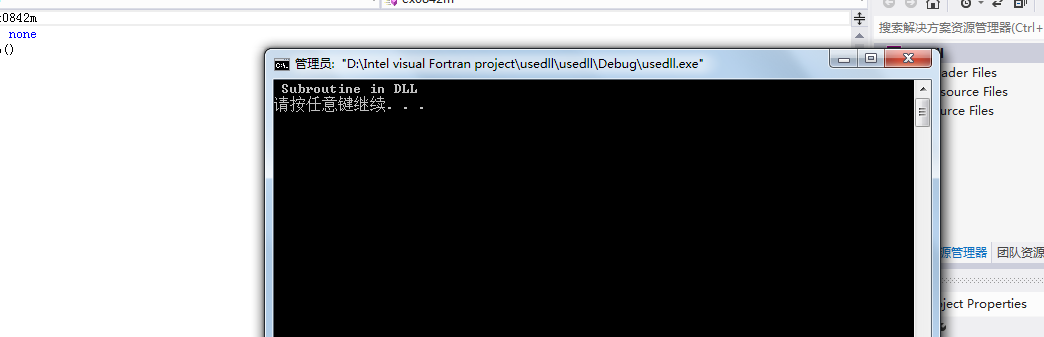
\includegraphics[scale=0.5]{11.png}
\caption{更改之前的运行结果。}
\end{figure}
\begin{figure}[ht]
\centering
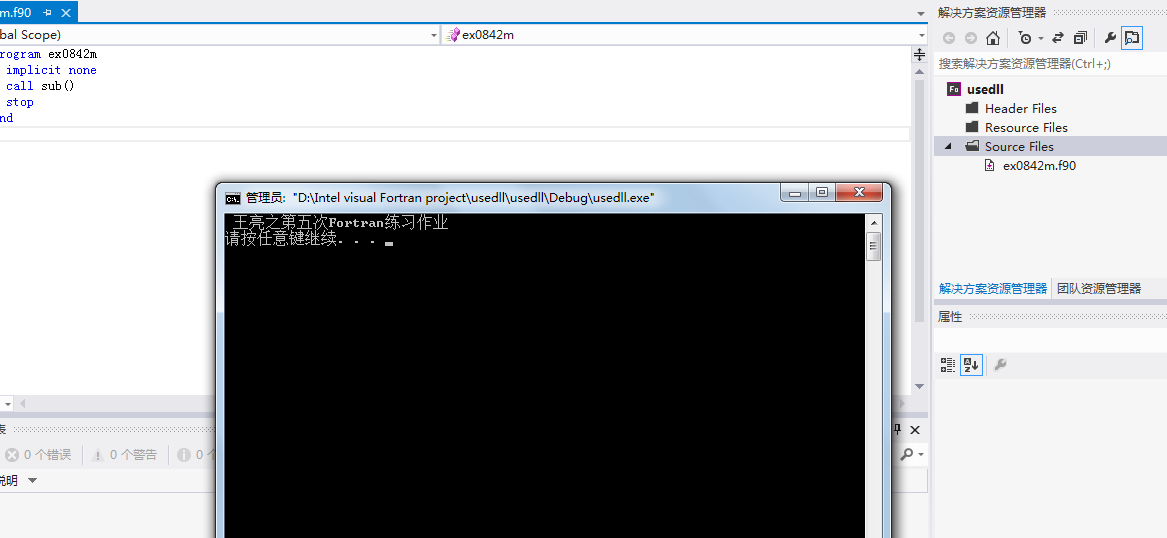
\includegraphics[scale=0.5]{王亮2.png}
\caption{更改之后的运行结果。}
\end{figure}
\section{考试题目}
编写徐世浙的《地球物理中的有限单元法》中108页的程序。计算子程序可直接使用书上给出的代码。主程序则自行编写。要求:
\begin{enumerate}
\item 程序需能计算出108页的数据结果(60分)
\begin{itemize}
\item 学生要能完成这项,必须会使用数组(第1章)和子程序(第3章)
\end{itemize}
\item 程序需实现数据与程序分离的编程原则:程序运行后再从文件录入输入值(15分)
\begin{itemize}
\item 学生要能完成这项,必须会使用文件(第4章)
\end{itemize}
\item 设计某种方式,给用户一个选择:如果得到肯定回答,则直接录入和教材例子完全相同的数据(这些数据可写在代码中,也可保存在文件中),进行计算(15分)
\begin{itemize}
\item 学生要能完成这项,必须会使用分支结构(第2章)
\end{itemize}
\item 程序录入数据后需向用户回显输入值(10分)
\end{enumerate}

\emph{本考试题目的源代码文件保存在pdf文件的附件中!}
\end{document}
